\documentclass[onecolumn, draftclsnofoot,10pt, compsoc]{IEEEtran}

\usepackage{graphicx}
\usepackage{url}
\usepackage{setspace}
\usepackage{geometry}
\usepackage{listings}
\usepackage{etoolbox}

\patchcmd{\thebibliography}{\section*{\refname}}{}{}{}

\geometry{textheight=9.5in, textwidth=7in}

% 1. Fill in these details
\def \CapstoneTeamName{			              			 PlanteR-GB}
\def \CapstoneTeamNumber{					           			 Group 64}
\def \GroupMemberOne{				           				Austin Hodgin}
\def \GroupMemberTwo{				           				Travis Hodgin}
\def \GroupMemberThree{			            Maximillian Schmidt}
\def\GroupMemberFour{		        	               Zach Lerew}
\def \CapstoneProjectName{	      	    Winter is Coming...}
\def \CapstoneSponsorCompany{		    Oregon State University}
\def \CapstoneSponsorPerson{		 			  				 Victor Hsu}

% 2. Uncomment the appropriate line below so that the document type works
\def \DocType{		%Problem Statement
				Requirements Document
				%Technology Review
				%Design Document
				%Progress Report
				}

\newcommand{\NameSigPair}[1]{\par
\makebox[2.75in][r]{#1} \hfil 	\makebox[3.25in]{\makebox[2.25in]{\hrulefill} \hfill		\makebox[.75in]{\hrulefill}}
\par\vspace{-12pt} \textit{\tiny\noindent
\makebox[2.75in]{} \hfil		\makebox[3.25in]{\makebox[2.25in][r]{Signature} \hfill	\makebox[.75in][r]{Date}}}}
% 3. If the document is not to be signed, uncomment the RENEWcommand below
\renewcommand{\NameSigPair}[1]{#1}

%%%%%%%%%%%%%%%%%%%%%%%%%%%%%%%%%%%%%%%
\begin{document}
\begin{titlepage}
    \pagenumbering{gobble}
    \begin{singlespace}
    	%\includegraphics[height=4cm]{coe_v_spot1}
        \hfill

        % 4. If you have a logo, use this includegraphics command to put it on the coversheet.
        %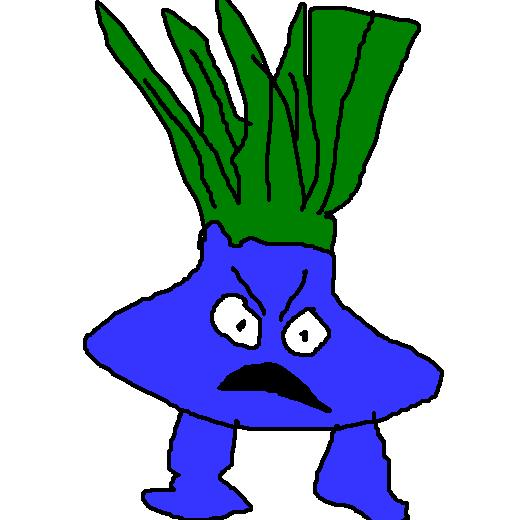
\includegraphics[height=4cm]{derp.jpg}

        \par\vspace{.2in}
        \centering
        \scshape{
            \huge CS Capstone \DocType \par
            {\large\today}\par
            \vspace{.5in}
            \textbf{\Huge\CapstoneProjectName}\par

            %\vfill
						\vspace{1in}

            {\large Prepared for}\par
            \Huge \CapstoneSponsorCompany\par
            \vspace{5pt}
            {\Large\NameSigPair{\CapstoneSponsorPerson}\par}

						\vspace{1in}

            {\large Prepared by}\par
						{\huge \CapstoneTeamNumber}\par
            \CapstoneTeamName\par
            \vspace{5pt}

            {
							\Large
							\NameSigPair{\GroupMemberOne}\par
							\NameSigPair{\GroupMemberTwo}\par
							\NameSigPair{\GroupMemberThree}\par
							\NameSigPair{\GroupMemberFour}\par
            }

            \vspace{20pt}
        }
%\textbf{\textsuperscript{citation needed}}
				\newpage
        \begin{abstract}
				\noindent This project will create a system that controls RGB LEDs responsible for indoor plant growth during the cold seasons.
				Seasonal weather conditions may vary between different parts of the world, but plant growth becomes especially difficult during the fall and winter months.
				Oregon is an exceptional case of this rule. The state's winter season produces a hostile growth environment for plants such as herbs, spices, and decorative flowers.
				Plants like these are not able to survive outside in the cold, dark, and humid Oregon weather.

				\noindent Bringing the plants into a more friendly and manageable indoor environment can still prove to be a difficult task.
				Plants need specific conditions for soil, water, temperature, and light.
				Existing indoor lighting systems can be difficult to use, expensive, and provide few customization options.
				Research provided by the client\cite[pg.4]{mark1}, has shown that some plants grow differently under different colors(wavelengths) of light.
				This project aims to produce a system that can control the color, intensity, and schedule for multiple zones of RGB LEDs.
				The system produced by these efforts will have a simple user interface through which all control settings can be viewed and manipulated.

				\noindent Once given control over the growing conditions, the plants will have a better chance of successful growth, and at the same time the impact on the user's busy life will be reduced.
				The system will be driven by a microcontroller that will manipulate the color, intensity, and schedule for multiple zones of RGB LEDs.
				Along side this hardware, the development of an intuitive user interface will allow the user to control the system with minimal physical interaction.
				The project has a simple core, but many stretch goals have been designed to increase functionality and end usability should time allow.

        \end{abstract}
    \end{singlespace}
\end{titlepage}

\newpage

\pagenumbering{arabic}
%\tableofcontents
% 7. uncomment this (if applicable). Consider adding a page break.
%\listoffigures
%\listoftables
\clearpage
\singlespace


	% Document body
	\section{Introduction}

		\subsection{Purpose}
			The goal of this document is to clearly list and define each of the requirements defined by the client.  Looking ahead, this will refine what the end result of the project shall be,
			such that the client's and team's expectations are fully met after all work is completed.  This document will also address any uncertainty about the end result of the proposed product,
			before work begins.
		\subsection{Scope}
			This document includes the requirements initially given by the client as interpreted by the team, the requirements and successive additions that the team has set to improve upon the initial client requirements, and the technical applications that will be used to cover each requirement.  Such requirements will mold the final product in its form and functionality.
			To detail each requirement, the team has provided technical specifics on how each requirement will be met.  The document also includes the details that the team will be executing step by step
			during the project to meet said result.

		\subsection{Definitions, Acronyms, and Abbreviations}
			LED - Light Emitting Diode \\
			RGB - Red, Green, Blue. Usually referring to a LED that is capable of producing those three colors. \\
			GPIO - General Purpose Input Output pins, allow the transfer of data between a microcontroller and an external piece of hardware. \\
			TCP - Transmission Control Protocol \\
			UDP - User Datagram Protocol \\
			REST - Representational state transfer \\
			API - Application Programming Interface \\

		% References
		\subsection{References}
		%\cite[Sec 3.8]{sourceName}
		\bibliographystyle{IEEEtran}
		\bibliography{./ref}


		\subsection{Overview}
			In accordance with the requirements laid out by the client and team, an overall description has been provided that will detail the specifics on what will be used.  The description will dive into
			the details of hardware and software that the team envisions the project will use to meet and exceed the requirements.  Version numbers, as well as internal iterations of the versions, will detail
			and divide each set of specifications and the application of the mentioned software and hardware.


	\section{Overall Description}
		\subsection{Product Perspective}

		\subsubsection{Product Functions}
		\noindent \textbf{Version 1.0} will consist of three major parts. The first part will be the programmable LEDs that will be used to light the plants. These will need to be reprogrammable in order to allow new settings.
		These settings include LED color on the RGB spectrum, intensity of the light, and the time the LEDs will turn on, and turn off. All LEDs in this version will be set to the same settings, meaning all
		LEDs will have the same color, intensity and light time. The second part will be the microcontroller. The microcontroller will allow the LEDs to be programed, and will provide power for early iterations.
		The third part is a user interface to allow these settings to be changed. This version will consist of a configuration file that can be manually changed to modify these settings.

		\noindent \textbf{Version 2.0} consists of additional features added by our team. Version 2.0 will require everything from Version 1.0 to be completed. This version will add many new features. The first, and most
		important feature will be an easier way to manage the settings. This version will add a web interface that will allow the user to change settings without having physical access to the controller.
		This new user interface will be able to display the current settings as well as allow the user to make changes. Further additions to the user interface include adding a mobile web page, and android
		phone support to allow users to update settings on their phone or other mobile device, further adding easier access to the settings. This version will also allow the user to change the LEDs to a new color or intensity for more flexibility. Adding moisture and temperature sensors is another goal for this version. Adding these will further allow the user to adjust
		their environment for the specific plants they are growing.

		\noindent \textbf{Version 3.0} consists of our stretch goals, goals that we will attempt to complete when we are finished with version 1.0 and 2.0, given we have enough time. This version, like the last version,
		requires all previous versions to be complete. Our first stretch goal will be to add predefined setting profiles for various plants. These include adding color, intensity and light timings optimized
		for various types of herbs, such as parsley vs basil. This further makes settings easier to manage for the user, taking much of the guess work or research out of the equation. Another stretch goal will be
		to add modular planter boxes. This goal intends to allow the user to add planters together using a single microcontroller. Further goals include to expand this set up to larger scale growing systems,
		such as greenhouses.


		\subsubsection{System Interfaces}
				The system as a whole serves as an arbitrator between a user and the ideal growth of their plants.
				The microcontroller will have control over a series of LEDs, including their color, intensity, and power schedule. The same microcontroller will host an interface that allows the user to control
				how the microcontroller adjusts the properties of its LEDs. Initially during iteration zero and one, the user interface to the system will be simplistic and require a high skill ceiling to use. As the project matures into iteration six, a more useful and
				simplistic interface will be developed. Similarly, the number of supported LEDs will be limited until iteration five when a better power management solution is made.
		 \subsubsection{User Interfaces}
				System properties will be controlled through a configuration file that is read by the control service and transformed into the appropriate GPIO signals to change the LED state. Starting at
				iteration one, the configuration file will be the primary and only way to interact with the system's properties. After core abilities are developed, iteration two will create a text-based command
				line menu system that allows all settings to be modified. This command line menu will be updated until iteration five, after which it will be replaced.
				The iteration six web interface will be hosted on the microcontroller and will communicate with the control service through changes to the configuration file. This interface will be clearly
				organized into categories for each of the major features (e.g. Zones, Scheduling, Profiles, manual control, etc).
			\subsubsection{Hardware}
				The microcontroller will be the brains for this system, and needs to be capable of running a service that controls the LEDs, as well as hosting a web server accessible from the local network.
				For iteration zero, the microcontroller must be capable of delivering enough power for a single LED strip. Iteration five will use a separate power supply, but the microcontroller must still control
				at least four LED strips. Iterations twelve and fifteen will require a separate power supply and regulator chip and possibly support data over USB to support larger lighting systems.
			\subsubsection{Software Interfaces}
				The control service is the bridge between the LEDs and the user interface, it will run on a microcontroller as a background service.
				In version 1.0, the user interface will be simplistic but functional. There will be a higher barrier of entry required to use these early interfaces, to allow the project to focus on the primary features of the system.
				After iteration five, a web interface will be developed. It will be hosted using a website hosting service such as Apache2. The web interface will use a simple tabular card based interface
				that will allow all system settings to be viewed and modified as the system is running.

			\subsubsection{Communications Interfaces}
				The control service will communicate with LEDs over the microcontroller's GPIO pins. Data transfer to the LEDs will occur over GPIO pins until iteration thirteen and higher which can bring support for a
				large amount of LEDs, but may require communication over USB.
				Iteration thirteen will bring support for communication between distributed systems over the TCP through a REST API built into the control service.
			\subsubsection{Memory Constraints}
				The memory constraints are determined by the type of programmable LED chosen and the type of microcontroller. Memory constraints will change as parts are specified and become part of the project.

			\subsubsection{Operations}
				The operations of this product change based on which iteration we are on. In the first iteration the user will be operating the system through a configuration file on the system. In the second iteration
				the way the user interacts with it changes to an interactive script. This script will ask questions about how the user would like to configure the system. Then makes the changes to the configuration file.
				The sixth iteration will then change the user operations again by allowing the user to make configurations using a web interface hosted by the system. With each step the system will apply changes from the configuration file in a steady interval (Instant, 5 sec, 10 sec, 30 sec). This is subject to change based on how long the control service takes to reload and apply the changes.
			\subsubsection{Site Adaptation Requirements}
				The system will change to support different number of LEDs, which are limited by software, depending on which iteration we are in. With iteration four, two zones will be controlled and powered by the microcontroller.
				In iteration five the amount of zone will increase to four zones powered by a separate power supply. With iterations twelve and fifteen another controller may be needed to push settings to the increased number of LEDs.


		\subsection{User Characteristics}
		Iterations zero and one will require the user to connect to the microcontroller, either physically, or through an SSH/FTP connection. Knowledge on how to traverse common folder systems will be needed for physical transfer, such as
		through an SD card or USB connection. SSH connections will require the user to know how to traverse a Unix terminal.
		Iteration two through five will require the user to know how to traverse a Unix terminal, as well as run a script. Users will further have to follow a list of questions and answer them with correct color, intensity, and time.
		Iteration five through fifteen will require the user to be able to connect to a website hosted by the microcontroller by connecting to its local host. The user will also need to know how to click buttons and go through drop down menus on the site.

		\subsection{Constraints}
		For iterations zero through four, we will be constrained to using only a max of ten LEDs, due to power limitations. For iterations five through ten, we will be constrained to powering the LEDs off a separate power supply than the microcontroller,
		since we may be using more than the max for iterations zero through four. We will have more constraints based on the microcontroller used. Certain controller will have more or less GPIO pins. Microcontrollers may have different clock speeds, and RAM sizes.

		\subsection{Assumptions and Dependencies}
		Each version and iteration requires that the previous versions and iterations be complete. Version 2.0 requires version 1.0 to be finished, and iteration five requires that iteration zero through four be finished.
		Through iteration five and onward, we will be working with more LEDs. Depending on the microcontroller, the LEDs may need to be powered separately from the controller itself, as they may draw too much current.
		Iteration twelve through fifteen will depend on a separate LED controller that will help facilitate the indexing of, and controlling of the LEDs. This also depends on the availability of such a controller.
		\subsection{Gant Chart}
		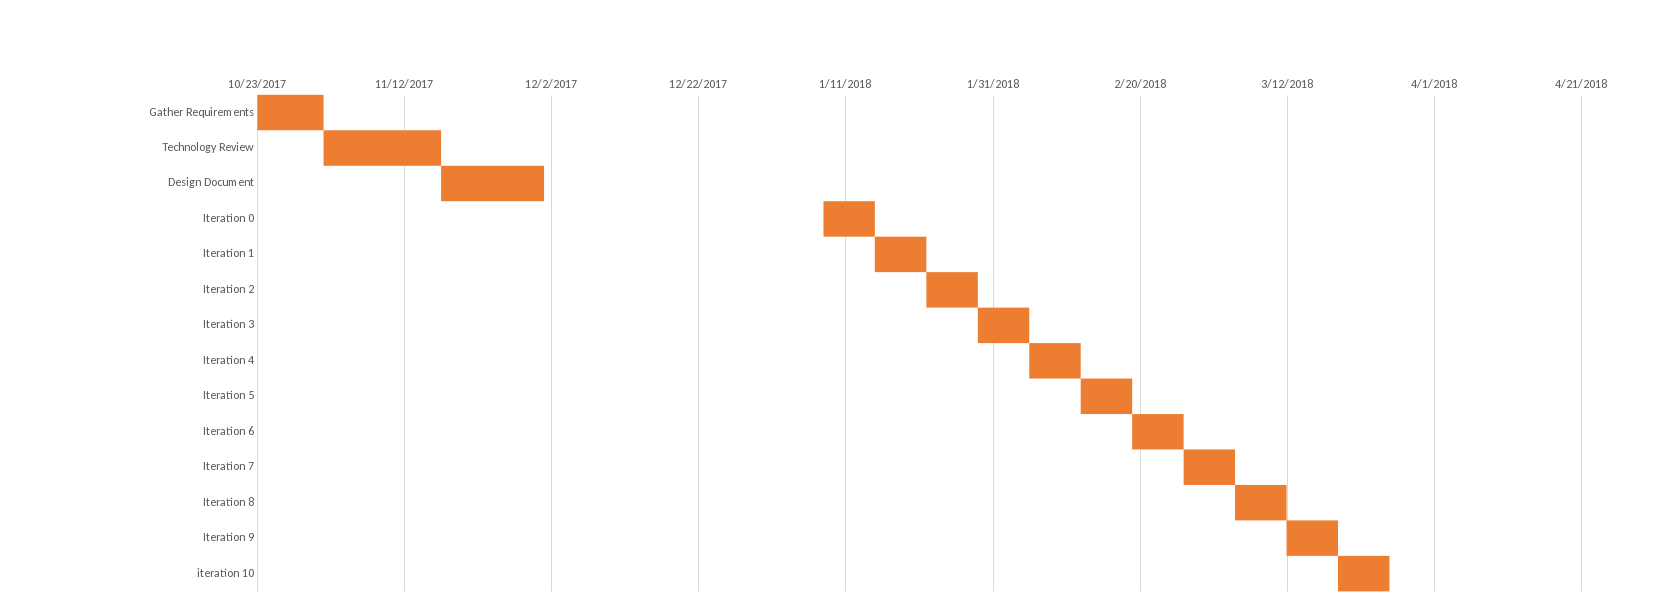
\includegraphics[width=\linewidth]{Gant.png}


	\section{Specific Requirements}
		\subsection{Required features - v1.0}
			\begin{itemize}
				\item Iteration 0
						\begin{itemize}
						\item A single LED strip with a single microcontroller intended to be used with a single planter
						\item Background service running on microcontroller which can communicate with LEDs through GPIO pins
						\item Control light color and intensity
					\end{itemize}
						\item Iteration 1
					\begin{itemize}
						\item Configuration settings for the light state is read from a configuration file
						\item Changes to the configuration file are recognized and applied by the controller at a regular interval
					\end{itemize}

				\item Iteration 2
					\begin{itemize}
						\item Simple user interface using command line script for basic control over settings
						\item All settings can be changed from this interface, though it may not be user friendly
					\end{itemize}
				\item Iteration 3
					\begin{itemize}
						\item User can specify weekly and daily scheduling for the state of the light (Color, Intensity, Power)
					\end{itemize}
				\item Iteration 4
					\begin{itemize}
						\item Light zoning - zones can be controlled and scheduled individually
						\item At least two zones supported and powered by microcontroller
					\end{itemize}
				\item Iteration 5
					\begin{itemize}
						\item Controller supports at least four and at most 20 zones, powered separately from the microcontroller
						\item Each zone can chain light strips together on one data pin due to strips being powered separately
					\end{itemize}
			\end{itemize}

		\subsection{Additional features - v2.0}
			\begin{itemize}
				\item Iteration 6
					\begin{itemize}
						\item Hosted web interface on local network
						\item Interface remains as simple as possible
						\item Shows the current state of the system
						\item Can modify all configuration settings of control service on local microcontroller
					\end{itemize}
				\item Iteration 7
					\begin{itemize}
						\item Sub zoning on an individual light strip
						\item Color and intensity set per LED
						\item LEDs grouped into zones, regardless of which strip they are on
					\end{itemize}
				\item Iteration 8
					\begin{itemize}
						\item Web interface adds support for mobile sized screens
						\item Android application acting as a wrapper for the web interface
					\end{itemize}
				\item Iteration 9
					\begin{itemize}
						\item Custom 3D printed planter with enclosure for controller, power supply, and LEDs
					\end{itemize}
				\item Iteration 10
					\begin{itemize}
						\item Humidity and temperature monitoring using additional hardware sensors
						\item Web interface support for humidity and temperature logging
					\end{itemize}
			\end{itemize}

		\subsection{Stretch goals - v3.0}
			\begin{itemize}
				\item Iteration 11
					\begin{itemize}
						\item Pre-built profile settings and per-plant settings that allow effortless light configurations to be applied that are specific to a particular plant species
					\end{itemize}
				\item Iteration 12
					\begin{itemize}
						\item Custom printed modular enclosure that allows multiple planters to be snapped together under a single controller
						\item Lights are automatically detected and zoned
					\end{itemize}
				\item Iteration 13
					\begin{itemize}
						\item Wireless “ad-hoc” style control over multiple distributed systems
						\item Control service will take input from a network protocol, allowing the web service to be run on a different local
					\end{itemize}
				\item Iteration 14
					\begin{itemize}
						\item Pre-setup OS/lighting system image for microcontroller, instruction guide for building your own system
						\item Kit with all necessary parts, pre-flashed system image
						\item Pre-built kit, plug and play, sold for profit
					\end{itemize}
				\item Iteration 15
					\begin{itemize}
						\item Support for very large distributed systems such as greenhouses
					\end{itemize}
			\end{itemize}

		\section{Performance Metrics}
		Defining performance metrics for this project has been a back and forth topic for this team. The client's requirements are easily met by a team of four people, but we have set our internal expectations are much higher. To avoid feature bloat and to guarantee the product functions per the client's requirements at a minimum, the features necessary to describe the project a success are a smaller subset of the overall features described in this document. This project is considered a success if: All features described in Version 1.0 are completed per specification and an alternative interface as described in iteration six is completed. Extra features will be added after the completion of these required
		features.


\end{document}
